%; whizzy section -pdf xpdf -latex ./whizzypdfptex.sh
% latex beamer presentation.
% platex, latex-beamer $B$G%3%s%Q%$%k$9$k$3$H$rA[Dj!%(B 

%     Tokyo Debian Meeting resources
%     Copyright (C) 2008 Junichi Uekawa

%     This program is free software; you can redistribute it and/or modify
%     it under the terms of the GNU General Public License as published by
%     the Free Software Foundation; either version 2 of the License, or
%     (at your option) any later version.

%     This program is distributed in the hope that it will be useful,
%     but WITHOUT ANY WARRANTY; without even the implied warranty of
%     MERCHANTABILITY or FITNESS FOR A PARTICULAR PURPOSE.  See the
%     GNU General Public License for more details.

%     You should have received a copy of the GNU General Public License
%     along with this program; if not, write to the Free Software
%     Foundation, Inc., 51 Franklin St, Fifth Floor, Boston, MA  02110-1301 USA

\documentclass[cjk,dvipdfm,12pt]{beamer}
\usetheme{Tokyo}
\usepackage{monthlypresentation}

%  preview (shell-command (concat "evince " (replace-regexp-in-string "tex$" "pdf"(buffer-file-name)) "&"))
%  presentation (shell-command (concat "xpdf -fullscreen " (replace-regexp-in-string "tex$" "pdf"(buffer-file-name)) "&"))

%http://www.naney.org/diki/dk/hyperref.html
%$BF|K\8l(BEUC$B7O4D6-$N;~(B
\AtBeginDvi{\special{pdf:tounicode EUC-UCS2}}
%$B%7%U%H(BJIS$B7O4D6-$N;~(B
%\AtBeginDvi{\special{pdf:tounicode 90ms-RKSJ-UCS2}}

\title{Debian Project and the Development Process, and how to co-work
with it.}
\subtitle{Cooperating with a large open source community}
\author{$B>e@n(B $B=c0l(B Junichi Uekawa\\dancer@debian.org\\IRC nick: dancerj}
\date{eeePC Developers' Conference 9 April 2008}
\logo{
\includegraphics[width=8cm]{image200607/openlogo-light.eps}}

\begin{document}

\frame{\titlepage{}}

% draft framework of talk.

\begin{frame}{}

This presentation is WIP.
\end{frame}

\begin{frame}{Junichi Uekawa}
\begin{itemize}
 \item Debian Developer since 2000
 \item Leading Debian JP Project since 2006
 \item Developer and maintainer of several Debian tools, such
       as pbuilder, dpatch, cowdancer, dsh, etc.
\end{itemize}
\end{frame}

\begin{frame}{What is Debian Project}
 \begin{itemize}%[<+->]
  \item 1 social contract, policy
  \item 11\footnote{etch official architectures} architectures 
  \item 215\footnote{as of 8 May 2008} mailing lists
  \item 1075\footnote{developers who can vote as of March 2008 DPL election}}
	maintainers 
	\footnote{2093 if including 755 with packages, 
	1338 sponsored people,  \url{http://io.debian.net/~tar/bugstats/?dancer\%40debian.org}}
  \item 10223\footnote{etch official source packages count, sid has 13574 as
	of 8 May 2008} packages
  \item All for Free Software.
 \end{itemize}
\end{frame}

\begin{frame}{What is Debian Distribution}
\begin{itemize}
 \item Debian GNU/Linux (i386) and Debian GNU/Linux (amd64) being the
       most used product.
 \item Not specific focus on Desktop or laptop or Server or embedded; tries to serve all.
 \item many architectures
 \item many kernels: Linux, kFreeBSD, Hurd....
\end{itemize}
\end{frame}

\begin{frame}{Debian Communication framework}
 \begin{itemize}
  \item mailing lists and archives (lists.debian.org)
  \item IRC network (irc.debian.org)
  \item BTS (bugs.debian.org)
  \item Wiki (wiki.debian.org)
  \item svn, Git, ... (alioth.debian.org, svn.debian.org,
	git.debian.org, ...)
 \end{itemize}
\end{frame}

\begin{frame}{Debian Development Process}

\includegraphics[width=1\hsize]{image200805/develcycle.eps} 

All processes are package-centric

\end{frame}

\begin{frame}{User Process: Install / Upgrade}
 \begin{itemize}
  \item new package: 
	user searches via apt-cache search, or finds out about package,
	and installs it via apt-get install / aptitude install / ...
  \item upgraded package:
	user upgrades package through 
	apt-get  / aptitude.	
 \end{itemize}
\end{frame}

\begin{frame}{User Process: the analysis workflow}
 \includegraphics[width=0.5\hsize]{image200805/problemcycle-en.eps}
\end{frame}

\begin{frame}{Tool: debconf}

Common interface to ask users questions.

 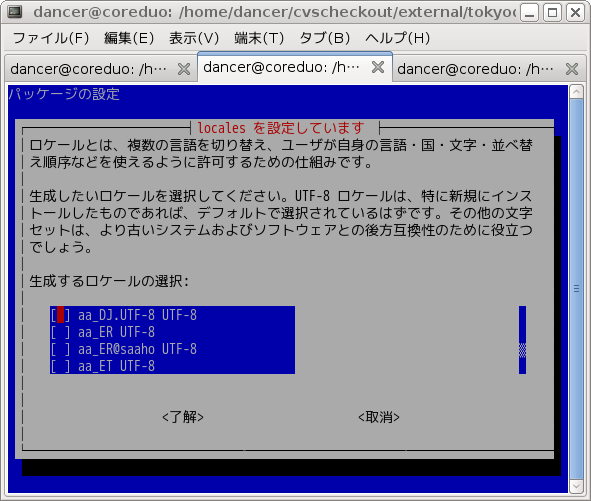
\includegraphics[width=0.5\hsize]{image200805/debconf-text.png}
 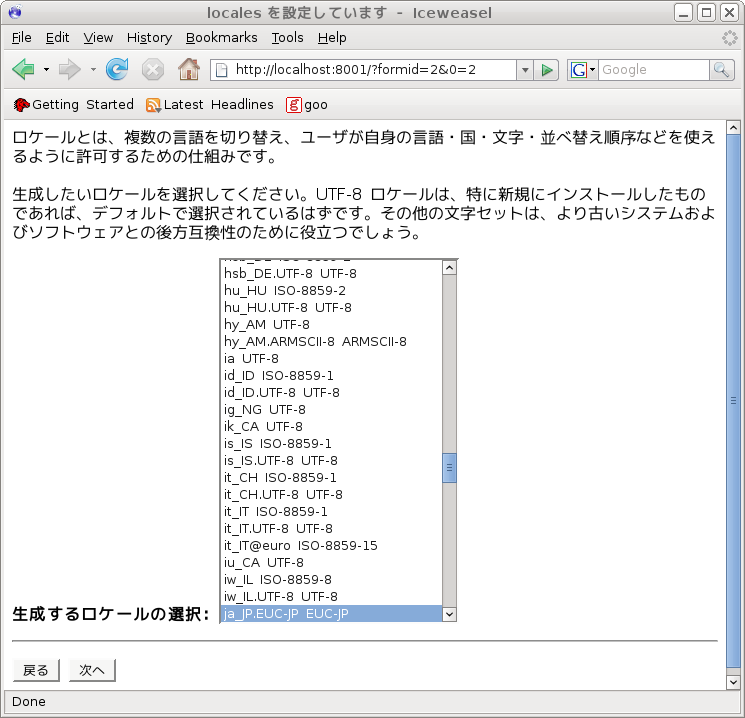
\includegraphics[width=0.5\hsize]{image200805/debconf-locales.png}

\end{frame}

\begin{frame}[containsverbatim]{Tool: apt-listbugs}
\begin{verbatim}
$B%P%0(B critical/dpkg (1.14.12 -> ) <done>
 #462104 - dpkg: [S-S-D] --pidfile and --retry seriously broken (dpkg/1.14.16.3 $B$G=$@5(B)
   $B0J2<$N%P%0$HE}9g$5$l$F$$$^$9(B: 462216
$B%P%0(B serious/apt (0.7.9 -> ) <done>
 #452862 - apt: FTBFS: dpkg-shlibdeps: failure: couldn't find library libapt-pkg-libc6.7-6.so.4.6 (apt/0.7.10 $B$G=$@5(B)
   $B0J2<$N%P%0$HE}9g$5$l$F$$$^$9(B: 453793 458396
$B%P%0(B serious/dpkg (1.14.12 -> ) <done>
 #461875 - dpkg: FTBFS: Can't locate Date/Parse.pm in @INC (dpkg/1.14.16.1 $B$G=$@5(B)
 #457962 - dpkg_1.14.13(m68k/unstable): Missing dependency on IO/String.pm (1.14.14 $B$G=$@5(B)
$BMWLs(B:
 apt(1 $B8D(B), dpkg(3 $B8D(B)
\end{verbatim}
\end{frame}


\begin{frame}[containsverbatim]{Tool: apt-listbugs}
\begin{verbatim}
critical bugs of cron (3.0pl1-86 -> 3.0pl1-87) <done>
 #282722 - Network install of Debian Woody Alpha -  cron corrupt on debian servers ?
grave bugs of strace (4.5.8-1.2 -> 4.5.9-1) <done>
 #294172 - strace - builds no s390 binary
grave bugs of gaim (1:1.1.2-3 -> 1:1.1.3-1) <done>
 #295904 - gaim: 1.1.3-1:  dies with SIGABRT on startup
grave bugs of reportbug (3.7.1 -> 3.8) <done>
 #295853 - reportbug includes sensitive information in report
grave bugs of cdbs (0.4.26-4 -> 0.4.27-1) <open>
 #295884 - cdbs: Changes control file to add new build dependency.
grave bugs of libdb4.3 (4.3.27-1 -> 4.3.27-2) <open>
 #294163 - libdb4.3: build failed on hppa
Summary:
 strace(1 bug), gaim(1 bug), cron(1 bug), cdbs(1 bug), libdb4.3(1 bug), reportbug(1 bug)
Are you sure you want to install/upgrade the above packages? [Y/n/?/...]
\end{verbatim}
\end{frame}

\section{apt-listchanges}
\begin{frame}[containsverbatim]{Tool: apt-listchanges}
\begin{minipage}{0.49\hsize}
 
 list changelog entries before install.

 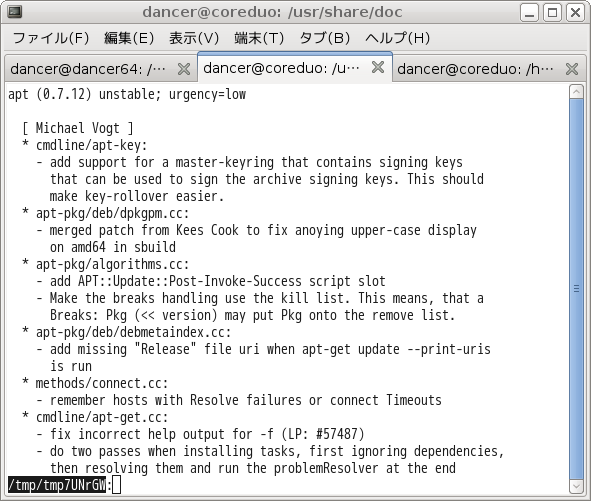
\includegraphics[width=1\hsize]{image200805/apt-listchanges.png}
\end{minipage}
\begin{minipage}{0.49\hsize}

\begin{commandline}
  dpkg-reconfigure apt-listchanges
\end{commandline} 
to make apt-listchanges to ask before installing

 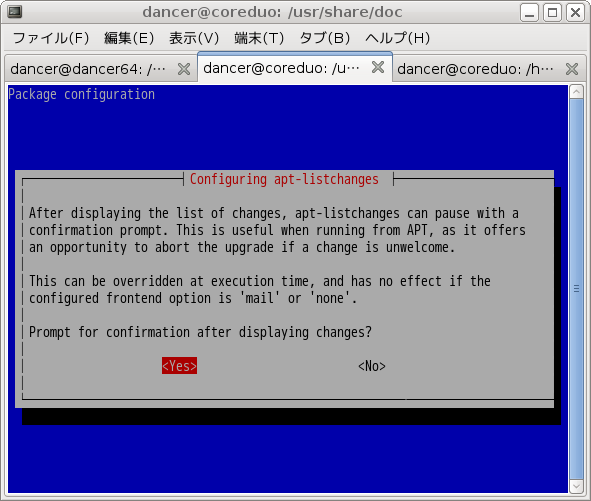
\includegraphics[width=1\hsize]{image200805/apt-listchanges-qa.png}
\end{minipage}
\end{frame}

\begin{frame}{User Process: using package}

where to find documentation.
where to find more information.
reading the policy to know what is expected.

\end{frame}

\begin{frame}{User Process: Problem Report 1/2}
\begin{itemize}
 \item Sending patches.
 \item Sending reproducible problem.
 \item Sending vague feature requests.
\end{itemize}

What do you want to do today?
\end{frame}

\begin{frame}{User Process: Problem Report 2/2}
Tools to use 
\begin{itemize}
 \item gdb, strace, valgrind, oprofile, etc ... 
 \item http://bugs.debian.org/ with Mail Interface
\end{itemize} 
\end{frame}

\begin{frame}{Tool: Bugs.debian.org interface}
Tools to use 
\begin{itemize}
 \item Mail interface.
 \item Web interface.
 \item GUI tools.
\end{itemize} 
\end{frame}


\begin{frame}[containsverbatim]{Tool: Bugs.debian.org interface: Mail}
\begin{minipage}{0.49\hsize}
\begin{itemize}
 \item The BTS commands work by e-mail (SMTP).
 \item Reading BTS is done via HTTP.
\end{itemize}
\end{minipage}
\begin{minipage}{0.49\hsize}
\begin{commandline}
To: submit@bugs.debian.org
Subject: Bug#429247: refit new upstream version
From: Junichi Uekawa <dancer@netfort.gr.jp>
Message-ID: <87odjgatfz.dancerj%dancer@netfort.gr.jp>

Package: refit
Version: 0.7

0.10 is released upstream, and is probably required for newer
hardware. However, gnu-efi in Debian currrently is too old to build
it.
\end{commandline}
\end{minipage}
\end{frame}

\begin{frame}{Tool: Bugs.debian.org interface: Web}

\includegraphics{image200508/bts.eps}
\end{frame}

\begin{frame}{Tool: Bugs.debian.org interface: TUI}
reportbug

 \includegraphics[width=1\hsize]{image200508/reportbug.eps}
\end{frame}

\begin{frame}{Tool: Bugs.debian.org interface: GUI}

reportbug-ng

 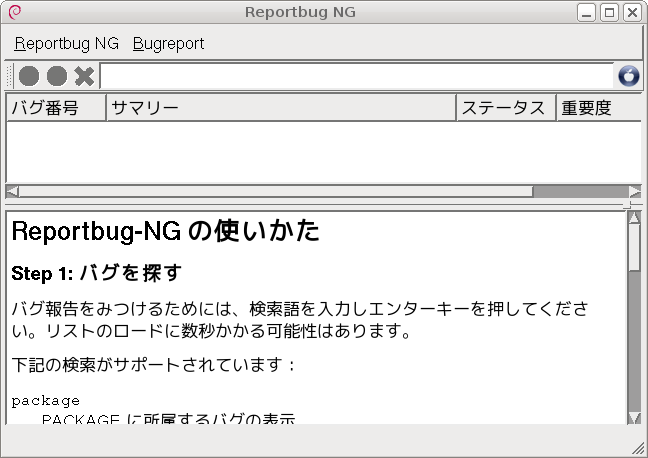
\includegraphics[width=1\hsize]{image200805/reportbug-ng.png}
\end{frame}

\begin{frame}{Developer Process: introduction}

 \includegraphics[width=0.5\hsize]{image200705/develcycle.eps}
\end{frame}

\begin{frame}{Developer Process: upload}

 \begin{itemize}
  \item new package 
  \item new upstream
  \item bug handling 
 \end{itemize}
\end{frame}

\begin{frame}{Developer Process: bug receive}
\end{frame}

\begin{frame}{Developer Process: bug analyse}

\end{frame}


\begin{frame}{Developer Process: bug fix}
\end{frame}

\begin{frame}{Developer Process: package upload}
\end{frame}

\begin{frame}{localization}
 There are different localization aspects. Looking at translation at
 random gives:
\begin{itemize}
 \item po: upstream translation, shared with other distributions etc.
 \item po-debconf: debconf prompt translation.
 \item debian.org, webwml: web page translation
 \item DDTP/DDTSS: Description translation
 \item po4a: tool to support translation
 \item i18n task force: \url{http://i18n.debian.net}
\end{itemize}
\end{frame}

\begin{frame}{localization: po editors}

    \includegraphics[width=0.4\hsize]{image200610/emacs-po.eps}
    \includegraphics[width=0.4\hsize]{image200610/kbabel.eps}

    \includegraphics[width=0.4\hsize]{image200610/gtranslator.eps}
\end{frame}

\begin{frame}{localization: po-debconf}

 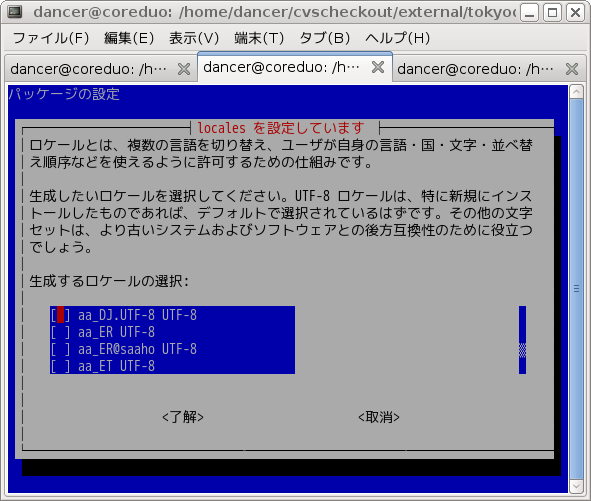
\includegraphics[width=0.5\hsize]{image200805/debconf-text.png}
 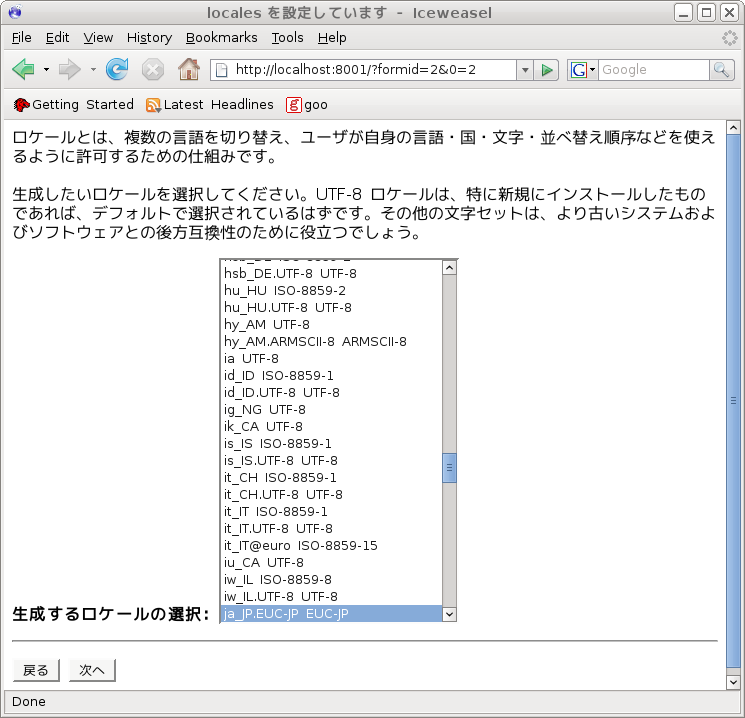
\includegraphics[width=0.5\hsize]{image200805/debconf-locales.png}

\end{frame}

\begin{frame}{i18n task force}
 \begin{itemize}
  \item i18n task force: \url{http://i18n.debian.net}
  \item IRC channel \url{\#debian-i18n@irc.debian.org}
 \end{itemize}
\end{frame}

\begin{frame}{Case study: Debian eeePC project}
 \begin{itemize}
  \item Porting Debian to eeePC
  \item Try to provide extra packages and integrate patches
  \item \url{http://wiki.debian.org/DebianEeePC}
 \end{itemize}
\end{frame}

\begin{frame}{What's Next}
 \begin{itemize}
  \item Taipei Debian Community Kick off 
	-- Be part of the next movement
  \item 10 May 2008 (Sat)
 \end{itemize}

\includegraphics[width=1\hsize]{image200712/debianmeetinganddebianjp.eps}
case of Japan

\end{frame}


\end{document}

;;; Local Variables: ***
;;; outline-regexp: "\\([ 	]*\\\\\\(documentstyle\\|documentclass\\|emtext\\|section\\|begin{frame}\\)\\*?[ 	]*[[{]\\|[]+\\)" ***
;;; End: ***
